\chapter{Практические приложения}
\label{cha:applications}

\section{Эволюция Шрамма-Левнера и алгебраические свойства предельного перехода от решеточных моделей к конформной теории поля}
\label{sec:SLE}

Эволюция Шрамма-Левнера появляется как скейлинговый предел интерфейсов в решеточных моделях в критической точке. Критическое поведение этих моделей можно описывать при помощи минимальных моделей конформной теории поля. Оказывается, что некоторые корреляционные функции в моделях конформной теории поля являются мартингалами по отношению к эволюции Шрамма-Левнера. 
В этой главе мы обобщаем эволюцию Шрамма-Левнера с дополнительным броуновским движением на группе Ли  $G$ на случай фактор-пространства $G/A$. Замет мы изучаем, как связано такое описание критического поведения с coset-моделями конформной теории поля. В качестве критерия согласованности мы используем тот факт, что минимальные модели могут быть реализованы как coset-модели при некотором выборе групп $G, A$.

\section{Введение}
Эволюция Шрамма-Левнера -- это стохастический процесс, который предложил Oded Schramm  \cite{schramm2000scaling} для описания скейлингового предела критических интерфейсов в двумерных статистических решеточных моделях. Этот подход к критическим системам дал много строгих результатов в теории критического поведения (см. обзоры  \cite{rohde2005basic}, \cite{bauer20062d}, \cite{Cardy:2005kh}). В разделе \ref{sec:schr-loewn-evol} мы приводим необходимые определения.  

Вероятностная мера, порожденная эволюцией Шрамма-Левнера на случайных кривых, конформно-инвариантна. Так как конформная теория поля представляет собой другой метод для изучения двумерных критических систем, естественно изучать ее связь с эволюцией Шрамма-Левнера. Такая связь изучалась, например, в работах \cite{bauer2004conformal,bauer2004cfts,bauer2003sle,bauer2002sle} (и многих других), но в основном для минимальных унитарных моделей. 
Идея состоит в рассмотрении определенных наблюдаемых в области с разрезом. Эта конструкция обсуждается в разделе \ref{sec:corr-betw-sle}. 

Более общие модели конформной теории поля обладают дополнительными симметриями. Например, алгебры Каца-Муди возникают в моделях Весса-Зумино-Новикова-Виттена.  Чтобы реализовать такие симметрии при изучении эволюции Шрамма-Левнера нужно ввести дополнительное случайное блуждание на группе Ли \cite{bettelheim2005stochastic}, \cite{Rasmussen:2004xr}. Такое случайное блуждание определяется в разделе \ref{sec:sle-wzw-models}. Соответствие между мартингалами эволюции Шрамма-Левнера и корреляционными функциями в моделях Весса-Зумино-Новикова-Виттена изучалось в работе \cite{alekseev2010sle}. Аналогичное обобщение на $\mathbb{Z}(N)$-парафермионную модель было предложено в статьях \cite{santachiara2008sle,picco2008numerical}. 

Основная задача данной главы состоит в обобщении эволюции Шрамма-Левнера с дополнительным случайным блужданием на группе Ли на случай фактор-пространства  $G/A$ и в изучении связи с coset-конструкцией конформной теории поля. В разделе \ref{sec:coset-models} мы напоминаем некоторые детали coset-конструкции, вводим эволюцию Шрамма-Левнера на фактор-пространстве и связываем ее с конформной теорией поля. По аналогии со случаем моделей Весса-Зумино-Новикова-Виттена мы получаем систему алгебраических уравнений на оператор смены граничного условия из условия на мартингал. 
При помощи coset-конструкции можно реализовать минимальные и парафермионные модели конформной теории поля (см. \cite{difrancesco1997cft}), так что мы можем сравнить наши уравнения на оператор смены граничных условий с результатами работы \cite{santachiara2008sle}.

В разделе  \ref{sec:conclusion} мы обсуждаем возможность сравнения классификации операторов смены граничных условий, следующей из свойства мартингалов с общей классификацией операторов смены граничных условий в граничной конформной теории поля, связанной с D-бранными решениями \cite{fuchs2005geometry,fredenhagen2002d,elitzur2002d,Maldacena:2001ky,felder1999geometry,alekseev1999d}. 

\subsection{Эволюция Шрамма-Левнера}
\label{sec:schr-loewn-evol}
Рассмотрим модель Изинга на треугольной решетке в верхней полуплоскости (см. Рисунок \ref{fig:sle}). Наложим следующее граничное условие: потребуем, чтобы на одной половине границы все спины были направлены вверх, а на другой половине -- вниз. Тогда при любой конфигурации спинов на полуплоскости будет интерфейс, разделяющий два кластера и соединяющий точку ноль с бесконечностью (см. Рисунок \ref{fig:sle}).

\begin{figure}[h]
  \centering{
    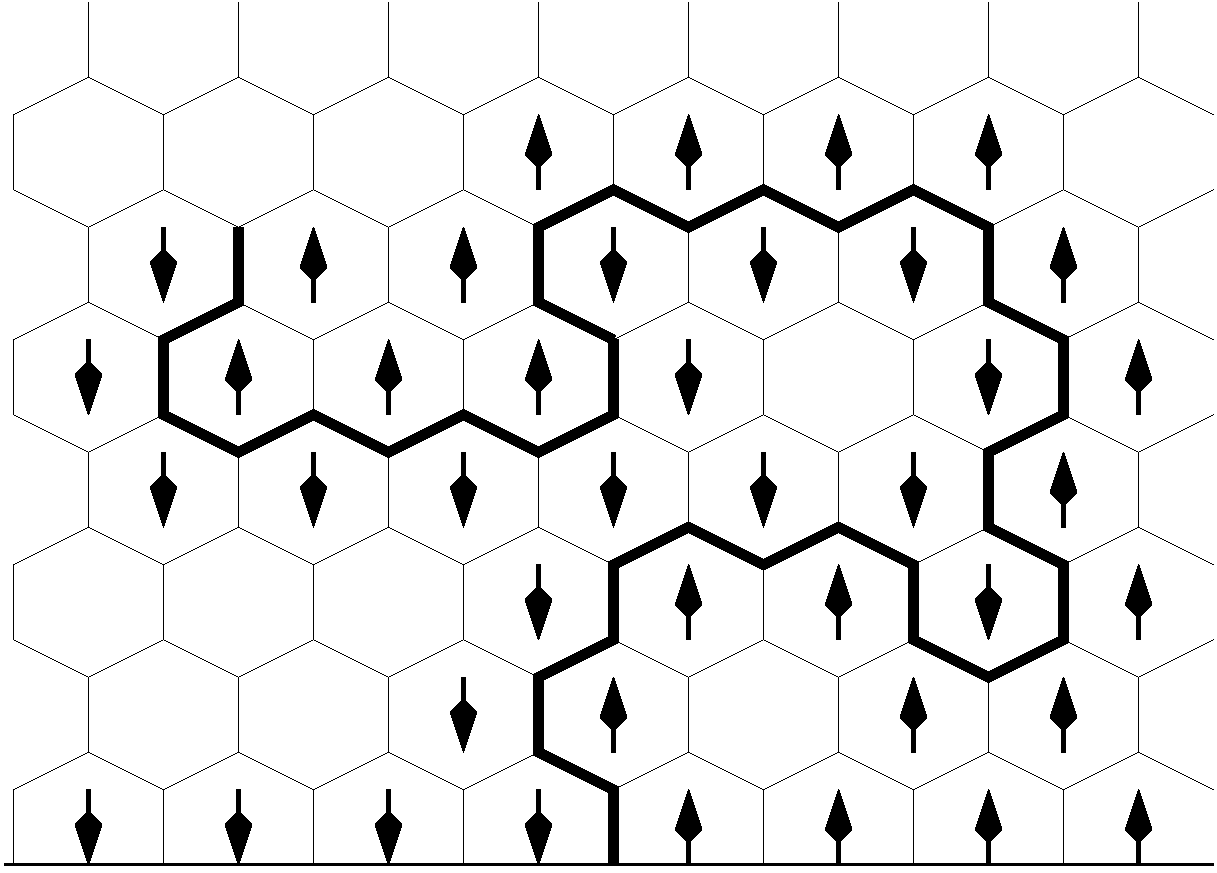
\includegraphics[height=50mm]{explore}
    \caption{Интерфейс в модели Изинга на треугольной решетке}}
  \label{fig:sle}
\end{figure}
Мы можем наложить условие существования части интерфейса конечной длины и рассмотреть конфигурации статистической модели, удовлетворяющие этому условию. Очевидно, такие конфигурации эквивалентны конфигурациям модели на области с разрезом вдоль интерфейса. 

Теперь рассмотрим непрерывный предел решеточной модели с (частью) интерфейса конечной длины. Интерфейсы в случайных конфигурациях модели сходятся к случайной кривой. Старая гипотеза \cite{Polyakov:1970xd} о конформной инвариантности в критической точке была недавно строго доказана для некоторых решеточных моделей (см. \cite{smirnov2007towards}, \cite{duminil2011conformal}). Мы предполагаем наличие конформной инвариантности в критической точке и рассматриваем верхнюю полуплоскость  $\mathbb{H}$ с разрезом вдоль критического интерфейса  $\gamma_{t}$. Такую область с разрезом мы обозначим через  $\mathbb{H}_{t}=\mathbb{H}\setminus \gamma_{t}$. Конформное отображение из $\mathbb{H}_{t}$ в $\mathbb{H}$ обозначим через $g_{t}:\mathbb{H}_{t}\to \mathbb{H}$ (см. Рисунок \ref{fig:sle2}).

\begin{figure}[h]
  \centering{
    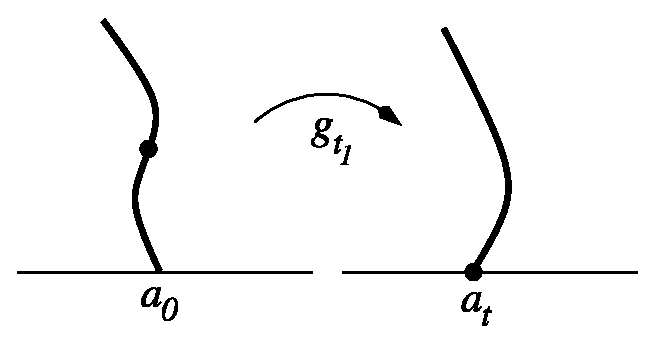
\includegraphics[width=60mm]{loewner}
    \caption{Конформное отображение $g_{t}(z):\mathbb{H}_{t}\to \mathbb{H}$.}}
  \label{fig:sle2}
\end{figure}

В статье \cite{schramm2000scaling} было показано, что  $g_{t}(z)$ удовлетворяет стохастическому дифференциальному уравнению
\begin{equation}
\label{eq:19}
  \frac{\partial g_t(z)}{\partial t} = \frac{ 2}{g_t(z)-\sqrt{\kappa}\xi_{t}} ,
\end{equation}
здесь $\xi_{t}$ -- Броуновское движение. Динамика конца  $z_{t}$ критической кривой $\gamma_{t}$ (конец следа эволюции Шрамма-Левнера) описывается уравнением $z_{t}=g_{t}^{-1}(\sqrt{\kappa}\xi_{t})$. 

Стохастический процесс, который удовлетворяет уравнению \eqref{eq:19} называется {\it эволюцией Шрамма-Левнера} на верхней полуплоскости $\mathbb{H}$. Для нас будет удобнее использовать отображение $w_{t} (z)=g_{t}(z)-\sqrt{\kappa}\xi_{t}$, так что уравнение \eqref{eq:19} переписывается в виде
\begin{equation}
  \label{eq:20}
       d w _{t}= \frac{2dt}{w_{t} }-\sqrt{\kappa}\xi_{t}  
\end{equation}
Эволюция Шрамма-Левнера порождает конформно-инвариантную вероятностную меру на кривых $\gamma_{t}$ в $\mathbb{H}$.

\subsection{Мартингалы эволюции Шрамма-Левнера и корреляционные функции в конформной теории поля}
\label{sec:corr-betw-sle}

Теперь рассмотрим наблюдаемые в присутствии следа эволюции Шрамма-Левнера. Математическое ожидание решеточной наблюдаемой $\mathcal{O}$ на верхней полуплоскости можно вычислить как сумму ожиданий этой наблюдаемой в присутствии (конечной части) траектории эволюции Шрамма-Левнера  $\gamma_{t}$ вплоть до некоторого времени $t$, умноженных на вероятность этой траектории:
\begin{equation*}
  \prec \mathcal{O} \succ_{\mathbb{H}}=\mathbb{E}\left[\prec\mathcal{O}\succ_{\gamma_{t}}\right]=\sum_{\gamma_{t}} P\left[C_{\gamma_{t}}\right] \prec \mathcal{O} \succ_{\gamma_{t}}
\end{equation*}
Решеточная наблюдаемая  $\prec \mathcal{O} \succ_{\mathbb{H}}$ не зависит от  $t$, следовательно $\prec\mathcal{O}\succ_{\gamma_{t}}$ -- мартингал.

В непрерывном пределе решеточные наблюдаемые сходятся к корреляционным функциям в конформной теории поля \cite{bauer2003sle,bauer2003conformal,bauer2002sle}. Мы должны учесть изменение граничных условий на конце следа эволюции Шрамма-Левнера и на бесконечности, так что соотношение имеет вид:
\begin{equation}
  \prec \mathcal{O} \succ_{\mathbb{H}_{t}}\to \mathcal{F}(\left\{z_{i}\right\})_{\mathbb{H}_{t}}=
  \frac{\left< \mathcal{O}(\{z_{i}\})\phi(z_{t})\phi^{\dagger}(\infty)\right>_{\mathbb{H}_{t}}}{\left<\phi(z_{t})\phi^{\dagger}(\infty)\right>_{\mathbb{H}_{t}}}
%% =
%%   \frac{\left<^{g_{t}}
%% \mathcal{O}\phi(\xi_{t})\phi^{\dagger}(\infty)\right>_{\mathbb{H}}}{\left<\phi(\xi_{t})\phi^{\dagger}(\infty)\right>_{\mathbb{H}}}
\label{eq:21}
\end{equation}

%% Here $\phi(z_{t})$ is a primary field corresponding to boundary condition changing operator.
%% We've used the conformal map $g_{t}$ to get the expression on the whole plane in equation \eqref{eq:21}.
Мы рассматриваем теорию с границей, так что мы должны использовать модели граничной конформной теории поля и накладывать соответствующие граничные условия \cite{cardy1984conformal,cardy1989boundary,cardy1991bulk}. В случае верхней полуплоскости корреляционные функции в граничной конформной теории поля могут быть переписаны как корреляционные функции для теории на всей плоскости, но с удвоенным числом полей.

% Here we are interested mainly in properties of boundary condition changing operator $\phi$. 

Мы предполагаем, что $\mathcal{F}$ содержит некоторый набор примарных полей  $\varphi_{\lambda_{i}}$ с конформными весами $h_{\lambda_{i}}$. Так как мы рассматриваем граничную конформную теорию поля, мы должны добавить объемные поля в сопряженных точках  $\bar z_{i}$. Для дальнейшего использования в моделях Весса-Зумино-Новикова-Виттена мы обозначим конформные веса этих сопряженных полей через $h_{\lambda_{i}^{*}}$. Кроме того, у нас есть операторы смены граничного условия   $\phi$ на конце следа эволюции Шрамма-Левнера и на бесконечности. Воспользуемся конформным отображением   $w(z):\mathbb{H}\setminus\gamma_{t}\to \mathbb{H}$, чтобы переписать выражение \eqref{eq:21} на верхней полуплоскости без разреза:
\begin{equation}
  \mathcal{F}(\left\{z_{i}\right\})_{\mathbb{H}_{t}}=\prod \left(\frac{\partial w(z_{i})}{\partial z_{i}}\right)^{h_{\lambda_i}} 
  \prod \left(\frac{\partial \bar w(\bar z_{i})}{\partial \bar z_{i}}\right)^{h_{\lambda^{*}_i}}
  \mathcal{F}(\left\{w_{i}, \bar w_{i}\right\})_{\mathbb{H}}
  \label{eq:1}
\end{equation}

Теперь нам нужно рассмотреть, как преобразуется конец следа эволюции Шрамма-Левнера  $\gamma_{t}$ при переходе от времени $t$ к $t+ dt$. Первый множитель в правой части уравнения  (\ref{eq:1}) дает нам
\begin{equation*}
  -\frac{2h_{\lambda_{i}}}{w_{i}^{2}}\left(\frac{\partial w_{i}}{\partial z_{i}}\right)^{h_{\lambda_{i}}}.
\end{equation*}
Для преобразования примарных полей  $\varphi_{\lambda_{i}}$ имеет место равенство
\begin{equation}
  \label{eq:2}
  d\varphi_{\lambda_{i}}(w_{i}) = \mathcal{G}_{i}\varphi_{\lambda_{i}}(w_{i})=\left(\frac{2dt}{w_{i}}-\sqrt{\kappa} d\xi_{t}\right) \partial_{w_{i}}\varphi_{\lambda_{i}}(w_{i}) 
\end{equation}
Мы обозначим генератор этого преобразования через  $\mathcal{G}_{i}$.

Так как $ \prec\mathcal{O}\succ_{\gamma_{t}}$ --  мартингал, математическое ожидание его приращения при эволюции от  $t$ к $t+dt$ равняется нулю
\begin{equation}
  \mathbb{E}\left[\prec\mathcal{O}\succ_{\gamma_{t}}\right]=    \mathbb{E}\left[\prec\mathcal{O}\succ_{\gamma_{t+dt}}\right], \quad d\mathbb{E}\left[ \prec\mathcal{O}\succ_{\gamma_{t}}\right]=0
\label{eq:22}
\end{equation}
Используем исчисление Ито и получим выражение для дифференциала $\mathcal{F}$:
\begin{equation}
d \mathcal{F}_{\mathbb{H}_{t}}= \left(\prod_{i=1}^{2N}\left(\frac{\partial w_{i}}{\partial z_{i}}\right)^{h_{i}}\right)\left(-\sum_{i=1}^{2N}\frac{2h_{i}dt}{w_{i}^{2}}+\left[\sum_{i=1}^{2N}\mathcal{G}_{i}+\frac{1}{2}
      \sum_{i,j}\mathcal{G}_{i}\mathcal{G}_{j}\right]\right)\mathcal{F}_{\mathbb{H}}=0
\label{eq:8}
\end{equation}
Подставим формулу \eqref{eq:2} и получим уравнение
\begin{equation}
  \left( \sum_{i}\left[-\frac{2h_{i}}{w_{i}^{2}} +\frac{2}{w_{i}}\partial_{w_{i}}\right]+\frac{\kappa}{2}\sum_{i,j}\partial_{w_{i}} \partial_{w_{j}}\right)\mathcal{F}(\left\{z_{i}\right\})=0
\label{eq:23}
\end{equation}

Для корреляционных функций вторичных полей  $L_{-n}\phi$ имеет место уравнение
\begin{equation}
\left< (L_{-n}\phi)(z) \varphi_{1}\dots \varphi_{N}\right>=\mathcal{L}_{-n}\left<\phi\varphi_{1}\dots\varphi_{N}\right>,
\end{equation}
где $n\geq 1$ и
\begin{equation*}
  \mathcal{L}_{-n}=\sum_{i=1}^{N} \left(\frac{(n-1)h_{i}}{(w_{i}-z)^{n}} -\frac{1}{(w_{i}-z)^{n-1}}\partial_{w_{i}}\right)
\end{equation*}
(См. \cite{difrancesco1997cft}). То есть мы можем переписать дифференциальное уравнение \eqref{eq:23} как алгебраическое уравнение на поле $\phi$, соответствующее оператору смены граничных условий:
\begin{equation}
  \label{eq:24}
   \left<\left([L_{-2}-\frac{\kappa}{2}L_{-1}^{2}]\phi\right)(0)\; \varphi_{\lambda_{1}}\dots \varphi_{\lambda_{{2N}}}\right>=0.
\end{equation}
В случае минимальных моделей набор примарных полей конечен и все состояния можно получить через соответствие между полями и состояниями
\cite{belavin1984ics}, \cite{difrancesco1997cft}. 
Равенство \eqref{eq:24} верно для произвольной наблюдаемой $\mathcal{O}$ и для произвольных примарных поле $\varphi_{\lambda_{i}}$, так что $\psi=[L_{-2}-\frac{\kappa}{2}L_{-1}^{2}]\phi$ -- нулевое поле уровня два и $\psi(0)\left|0\right>$ -- нулевое состояние уровня два. В минимальных унитарных моделях существует только два примарных поля, порождающих модули Верма алгебры Вирасоро с нулевыми состояниями на уровне два. Это поля $\phi_{1,2}$ и $\phi_{2,1}$, так что $\phi\sim \phi_{1,2} \;\text{or}\; \phi_{2,1}$. 

\section{Wess-Zumino-Novikov-Witten models}
\label{sec:sle-wzw-models}
To generalize the analysis of previous section \ref{sec:corr-betw-sle} to non-minimal models we need to take into account extra symmetries. Wess-Zumino-Novikov-Witten models has Kac-Moody symmetry in addition to conformal invariance leading to the appearance of Virasoro algebra. At first we remind well-known properties of WZNW-models \cite{difrancesco1997cft} which are useful to study SLE martingales. 

 The action of WZNW model can be written in terms of map $g:\mathbb{C}\cup \{\infty\}\sim S^{2}\to G$ from complex plane with infinity or two-sphere to some (simple) Lie group $G$:
\begin{multline}
  S=-\frac{k}{8\pi}\int d^2x\; \mathcal{K} (g^{-1}\partial^{\mu}g, g^{-1} \partial_{\mu}g)  
  - \frac{k }{24\pi^{2}} \int_{B}\epsilon_{ijk} \mathcal{K}\left(
    \tilde g^{-1}\frac{\partial \tilde g}{\partial y^i},\left[
      \tilde g^{-1}\frac{\partial \tilde g}{\partial y^j}
      \tilde g^{-1}\frac{\partial \tilde g}{\partial y^k}\right]\right) d^3y
\end{multline}
 Here $\mathcal{K}$ is Killing form on Lie algebra $\gf$ of Lie group $G$. The first term is just non-linear sigma-model and the second term is written using the continuation $\tilde{g}$ from two-sphere $S^{2}$ to three-dimensional manifold $B$ which has two-sphere as the boundary. Since this continuation is non-unique we get the requirement for $k$ to be integer. 

Conserved currents of this model have the following form:
  \begin{eqnarray}
    J(z)= -k \partial_zg g^{-1}
    \bar J(\bar z)=k g^{-1}\partial_{\bar z}g
  \end{eqnarray}

The model possesses gauge invariance under the transformations
  $g(z,\bar z)\to \Omega(z)g(z,\bar z)\bar \Omega^{-1}(\bar z)$, 
where $\Omega,\;\bar \Omega \in G$ are are independent. If we consider infinitesimal gauge transformation $\Omega=1+\omega$ we get Ward identities 
  \begin{equation}
    \label{eq:87}
    \delta_{\omega,\bar \omega}\left< X \right>=-\frac{1}{2\pi i}\oint dz \sum\omega^a \left< J^a X\right>+
    \frac{1}{2\pi i} \oint d\bar z \sum \bar \omega^a \left< \bar J^a X\right>,
  \end{equation}
which can be used to get operator product expansion for currents:
 \begin{equation}
   \label{eq:3}
   J^{a}(z)J^{b}(w)\sim \frac{k\delta_{ab}}{(z-w)^{2}}+\sum_{c}i f_{abc}\frac{J^{c}}{z-w},
 \end{equation}
where $f_{abc}$ are the structure constants of Lie algebra $\gf$.
 
Expanding the currents to modes
$J^a(z)=\sum\limits_{n\in \mathbb Z}z^{n-1}J^a_n $
and using operator product expansion \eqref{eq:3} we get commutation relations of affine Lie algebra $\gfh$:
\begin{equation*}
 \left[J^a_n,J^b_m\right]=\sum_c i f^{abc}J^c_{n+m}+kn\delta^{ab}\delta_{n+m,0}.  
\end{equation*}


Conformal invariance of the model can  be seen from 
Sugawara construction, which is a way to embed Virasoro algebra into the universal enveloping algebra of affine Lie algebra $\gfh$ ($Vir\subset U(\gfh)$):
\begin{equation}
  \label{eq:4}
  L_n=\frac{1}{2(k+h^{\vee})}\left(\sum\limits_a\sum\limits_{m\leq -1}J^a_m J^a_{n-m}+\sum_{m\geq 0} J^{a}_{n-m}J^{a}_{m}\right), 
\end{equation}
 where $h^{\vee}$ is the dual Coxeter number of Lie algebra $\gf$. 
Full chiral algebra of the model is semidirect product of affine and Virasoro algebra $\gfh \ltimes Vir$ with commutation relations 
  \begin{equation}
    \label{eq:92}
    \begin{aligned}
      \left[J^a_n,J^b_m\right]=\sum_c i f^{abc}J^c_{n+m}+kn\delta^{ab}\delta_{n+m,0} \\
      \left[L_n,L_m\right]=(n-m)L_{n+m}+\frac{c}{12}(n^3-n)\delta_{n+m,0}\\
      \left[L_n,J^a_m\right]=-mJ^a_{n+m}
    \end{aligned}
  \end{equation}
Here central charge $c$ of Virasoro algebra is given by expression
\begin{equation}
  \label{eq:25}
  c=\frac{k\;\mathrm{dim}\gf}{k+h^{\vee}}
\end{equation}
There is infinite number of Virasoro primary fields, but they are organized into highest weight modules of affine Lie algebra $\gfh$. 
Primary fields of full chiral algebra $\phi_{\lambda}$ are labeled by highest weights of  $\gfh$-modules. Here we see how Virasoro and affine Lie algebra generators act on primary fields:
  \begin{equation*}
    \begin{aligned}
      & J_0^a\left|\phi_{\lambda}\right>=-t^a_{\lambda}\left|\phi_{\lambda}\right>  \quad    J^a_n\left|\phi_{\lambda}\right>=0 \quad \mbox{for}\; n>0 \\
      & L_0\left|\phi_{\lambda}\right>=\frac{1}{2(k+h^{\vee})}\sum_aJ^a_0J^a_0\left|\phi_{\lambda}\right>=\frac{(\lambda,\lambda+2\rho)}{2(k+h^{\vee})}\left|\phi_{\lambda}\right>=h_{\lambda} \left|\phi_{\lambda}\right>,
    \end{aligned}
  \end{equation*}
where $\rho$ is Weyl vector of $\gf$. 

Now we want to study Schramm-Loewner evolution in WZNW-models.
Similarly to minimal models we consider observable
\begin{equation*}
  \mathcal{F}(\left\{z_{i}\right\})_{\mathbb{H}_{t}}=
  \frac{\left<\phi_{\Lambda}(z_{t}) \phi_{\lambda_1}(z_{1}) \dots \phi_{\lambda_n}(z_{n}) \phi_{\lambda^{*}_1}(\bar z_{1}) \dots \phi_{\lambda^{*}_n}(\bar z_{n})
      \phi_{\Lambda^{*}}(\infty)\right>}{\left<\phi_{\Lambda}(z_{t})\phi_{\Lambda^{*}}(\infty)\right>}
\end{equation*}
Again we can use conformal map  $w(z):\mathbb{H}\setminus\gamma_{t}\to \mathbb{H}$ to rewrite it on the whole upper half-plane. 
\begin{equation*}
  \mathcal{F}(\left\{z_{i}\right\})_{\mathbb{H}_{t}}=\prod \left(\frac{\partial w(z_{i})}{\partial z_{i}}\right)^{h_{\lambda_i}} 
  \prod \left(\frac{\partial \bar w(\bar z_{i})}{\partial \bar z_{i}}\right)^{h_{\lambda^{*}_i}}
  \mathcal{F}(\left\{w_{i}, \bar w_{i}\right\})_{\mathbb{H}}
\end{equation*}

Under the evolution from $t$ to $t+dt$ first factor gives us $-\frac{2h_{\lambda_{i}}}{w_{i}^{2}}\left(\frac{\partial w_{i}}{\partial z_{i}}\right)^{h_{\lambda_{i}}}$.

When we consider fields we need to add random gauge transformation (random motion in $G$) to stochastic evolution \cite{bettelheim2005stochastic}, \cite{alekseev2010sle}. 
For fields we have
\begin{equation*}
  d\phi_{\lambda_{i}}(w_{i}) = \mathcal{G}_{i}\phi_{\lambda_{i}}(w_{i}),
\end{equation*}
so additional term appears in the generator of field transformation. 
\begin{equation}
  \mathcal{G}_{i}=\left(\frac{2dt}{w_{i}}-\sqrt{\kappa} d\xi_{t}\right) \partial_{w_{i}}+\frac{\sqrt{\tau}}{w_{i}}\sum_{a=1}^{\mathrm{dim} \gf}\left(d \theta ^{a} t^{a}_{i}\right)
\label{eq:18}
\end{equation}
Here $d\theta^{a}$ are the generators of $\mathrm{dim}\gf$-dimensional Brownian motion and $\mathbb{E}[d\theta^{a}d\theta^{b}]=\delta_{ab}dt$. We assume that $t^{a}$ is a basis of $\gf$ orthogonal with respect to Killing form $\mathcal{K}$, $\mathcal{K}(t^{a},t^{b})=\delta_{ab}$.

Using formula \eqref{eq:8} we get the equation from martingale condition:
\begin{equation}
  \left(-2 \mathcal{L}_{-2}+\frac{1}{2}\kappa \mathcal{L}_{-1}^{2}+\frac{1}{2}\tau\sum_{a} \mathcal{J}^{a}_{-1} \mathcal{J}^{a}_{-1}\right)        \mathcal{F}(\left\{w_{i}, \bar w_{i}\right\})_{\mathbb{H}}=0,
  \label{eq:27}
\end{equation}
where
\begin{equation*}
  \mathcal{L}_{-n}=\sum_{i}\left(\frac{(n-1)h_{\lambda_{i}}}{(w_{i}-z)^{n}}-\frac{1}{(w_{i}-z)^{n-1}}\partial_{w_{i}}\right);\quad \mathcal{J}^{a}_{{-n}}=-\sum_{i}\frac{t^{a}_{i}}{(w_{i}-z)^{n}}
\end{equation*}
Again we can rewrite it as algebraic requirement for  field  which corresponds to boundary condition changing operator. Now
\begin{equation}
  \left| \psi\right>=\left(-2 L_{-2}+\frac{1}{2}\kappa L_{-1}^{2}+\frac{1}{2}\tau\sum_{a} J^{a}_{-1} J^{a}_{-1}\right) \left|\phi_{\Lambda}\right>    
  \label{eq:16}
\end{equation}
is level two null state and if we act on this state with raising operators we should get zero.
\begin{eqnarray}
  J^{a}_{1} \left|\psi\right>=0\\
  J^{a}_{2}\left|\psi\right>=0\\
  L_{2}\left|\psi\right>=0\\
  L_{1}\left|\psi\right>=0
\end{eqnarray}
Using commutation relations \eqref{eq:92} these equations can be rewritten as the algebraic equations connecting parameters of random motion $\kappa, \tau$ with the level $k$ of affine Lie algebra representation. Rigorous analysis of these equations is given in the paper \cite{alekseev2010sle}.

\section{Coset models}
\label{sec:coset-models}
Now we want to generalize analysis of correspondence between SLE and CFT even further and study coset models of conformal field theory\cite{Goddard198588}. Such models are specified by  Lie algebra $\gf$ and its subalgebra $\af$. Denote by $J_{n}^{a}$ the generators of affine Lie algebra $\gfh$ and by $\tilde{J}_{n}^{b}$ the generators of $\afh$, so that $\tilde{J}^{b}_{n}=\sum_{a} m_{a}^{b} J^{a}_{n}$.
Virasoro generators in coset models are given by the difference of Sugawara expressions of $\gf$ and $\af$-WZNW models:
\begin{equation*}
  L_{n}=L_{n}^{\gf}-L_{n}^{\af}
\end{equation*}
Commutation relations of Virasoro generators with generators of subalgebra $\afh$ are trivial
\begin{equation}
  \label{eq:26}
  \left[L_{n},\tilde{J}^{b}_{m}\right]=0
\end{equation}

Coset models can be realized as gauged Wess-Zumino-Novikov-Witten models by adding gauge fields  $A, \bar{A}$ taking values in Lie algebra $\af\subset \gf$ to the action\cite{gawdzki1988g}. Then fields are labeled by pairs of weights $(\mu,\nu)$, where $\mu$ is the weight of $\gfh$ and $\nu$ is the weight of $\afh$ correspondingly. But there are selection rules, i.e. the branching functions for certain pairs of weights $(\mu,\nu)$ vanish. There is also a redundancy, i.e. non-vanishing branching functions for distinct pairs $(\mu,\nu)$ turn out to be identical \cite{fuchs1996resolution,schellekens1990field}.

So, primary fields are labeled by pairs of weights $(\mu,\nu)\in \hf_{\gfh}\oplus \hf_{\afh}$  of algebra $\gfh$ and subalgebra $\afh$, such that branching functions $b^{\mu}_{\nu}(q)\neq 0$. Some pairs are equivalent. This equivalence is given by the action of so called ``simple currents'' $(J,\tilde{J})$, which are certain elements of outer  automorphisms group $\mathcal{O}(\gfh)\times \mathcal{O}(\afh)\approx B(G)\times B(A)$ of $\gfh\times\afh$, where $B(G)$ is center of Lie group G. We can think of simple currents as of primary fields and their action on fields of theory are then given by fusion product \cite{difrancesco1997cft}.  So primary fields of coset model are given by the equivalence classes of pairs of weights $(\mu,\nu)\sim (J*\mu,\tilde{J}*\nu)$, where $(J,\tilde J)$ such that their conformal weights are equal:  $h_{J}-h_{\tilde{J}}=0$. 

Conformal weight of coset primary field is equal to
\begin{multline}
  L_0\left|\phi_{(\mu,\nu)}\right>=\left(\frac{1}{2(k+h^{\vee})}\sum_aJ^a_0J^a_0-\frac{1}{2(k+h_{\af}^{\vee})}\sum_b \tilde{J}^b_0 \tilde{J}^b_0 \right)
  \left|\phi_{(\mu,\nu)}\right>=\\
  \left(\frac{(\mu,\mu+2\rho)}{2(k+h^{\vee})}-\frac{(\nu,\nu+2\rho_{\af})}{2(k+h^{\vee})}\right)\left|\phi_{(\mu,\nu)}\right>
\end{multline}
It is possible to obtain analogues of Knizhnik-Zamolodchikov equations for coset models \cite{kogan1997knizhnik}:
\begin{equation}
  \left\{\frac{1}{2}\partial_{i} + \sum_{i\neq j}^{N}\left(\frac{t^{a}_{i}t^{a}_{j}}{k+h^{\vee}}-\frac{\tilde t^{b}_{i}\tilde t^{b}_{j}}{k+h^{\vee}_{\af}}\right)\frac{1}{z_{i}-z_{j}}\right\} \left<\phi_{1}(z_{1})\dots \phi_{N}(z_{N})\right>=0
  \label{eq:6}
\end{equation}

Let us introduce Schramm-Loewner evolution corresponding to coset models. 
The idea is to constrain additional Brownian motion on group manifold to the factor space $G/A$. 


To study SLE on $G/A$ factor space we restrict random walk on group manifold by the choice of basis in $\gf$. Assume that generators $\{J^{a};\; a=1\dots \mathrm{dim}\gf\}$ are chosen in such way that $\mathcal{K}(J^{a},J^{b})=h^{\vee}\delta_{ab}$ and $\{J^{a};\; a=\mathrm{dim}\gf-\mathrm{dim}\af\dots \mathrm{dim}\gf\}$ are the generators of subalgebra $\af\subset \gf$. Now we can consider $(\mathrm{dim}\gf-\mathrm{dim}\af)$-dimensional Brownian motion with generators $d\theta^{a}$ such that $\mathbb{E}(d\theta^{a} \; d\theta^{b})=\delta_{ab};\; a,b=1,\dots,\mathrm{dim}\gf-\mathrm{dim}\af$.

Then for generator of field transformation we can write 
\begin{equation}
  \mathcal{G}_{i}=\left(\frac{2dt}{w_{i}}-\sqrt{\kappa} d\xi_{t}\right) \partial_{w_{i}}+\frac{\sqrt{\tau}}{w_{i}}\left(\sum_{a=1}^{\mathrm{dim}\gf-\mathrm{dim}\af}\left(d \theta ^{a} t^{a}_{i}\right)\right)
\label{eq:5}
\end{equation}
Substituting to equation \eqref{eq:8} we get martingale condition

\begin{equation}
  \left(-2 \mathcal{L}_{-2}+\frac{1}{2}\kappa \mathcal{L}_{-1}^{2}+\frac{\tau}{2}\left( \sum_{a=1}^{\mathrm{dim}\gf-\mathrm{dim}\af} \mathcal{J}^{a}_{-1} \mathcal{J}^{a}_{-1}\right)\right)        \mathcal{F}_{\mathbb{H}}=0
\label{eq:9}
\end{equation}

which can be rewritten as the requirement for
\begin{equation}
  \psi=\left(-2L_{-2}+\frac{1}{2}\kappa L_{-1}^{2}+\frac{1}{2}\tau \left(\sum_{a=1}^{\mathrm{dim}\gf-\mathrm{dim}\af}J^{a}_{-1}J^{a}_{-1}\right)\right) \phi_{(\mu,\nu)}
\label{eq:10}
\end{equation}
to be level two null-field. 

Now consider simple example. Let $G=SU(2)$ and $A=U(1)$, and corresponding Lie algebras $\gf=\mathrm{su}(2)$
with generators $J^{1},J^{2},J^{3}$ and $\af=\mathrm{u}(1)$ with the generator $J^{3}$, $\af\subset\gf$. Note that $\mathcal{K}(J^{a},J^{b})=2\delta^{ab}$. 
%%We label weights by Dynkin labels, so $J^{3}_{0}\phi_{(\mu,\nu)}=\frac{\mu}{2} \phi_{(\mu,\nu)}$.

 The equation \eqref{eq:10} is now
\begin{equation}
  \label{eq:11}
  \psi=\left(-2L_{-2}+\frac{1}{2}\kappa L_{-1}^{2}+\frac{1}{2}\tau \left(J^{1}_{-1}J^{1}_{-1}+J^{2}_{-1}J^{2}_{-1}\right)\right) \phi_{(\mu,\nu)}
\end{equation}
If we use basis $J^{+}=\frac{J^{1}+iJ^{2}}{\sqrt{2}},\; J^{-}=\frac{J^{1}-iJ^{2}}{\sqrt{2}}$ this equation is rewritten in the form
\begin{equation}
 \psi= \left(-2 L_{-2}+\frac{\kappa}{2}L_{-1}^{2}+\frac{\tau}{2}\left[J^{+}_{-1}J^{-}_{-1}+J^{-}_{-1}J^{+}_{-1}\right]\right) \phi_{(\mu,\nu)}
\label{eq:12}
\end{equation}
which is similar to the equations for parafermionic fields introduced in paper \cite{santachiara2008sle}.

Central charge in this case is equal to
\begin{equation}
  \label{eq:14}
  c=\frac{2(k-1)}{k+2}
\end{equation}

Let us study the solutions of the equation \eqref{eq:11}. Act on $\psi$ with $L_{2}$:
\begin{equation}
  \label{eq:13}
  L_{2}\psi=(-8L_{0}+c+3\kappa L_{0}+\tau k)\phi_{(\mu,\nu)}=0,
\end{equation}
and obtain
\begin{equation}
  \label{eq:28}
  (3\kappa-8) h_{(\mu,\nu)}+c+\tau k =0
\end{equation}
Another equation can be obtained by action of $L_{1}^{2}$
\begin{equation}
  \label{eq:15}
  L_{1}^{2}\psi = (12 L_{0} + \kappa(4 L_{0}^{2}+2 L_{0}) +\tau (J_{0}^{1}J_{0}^{1}+J_{0}^{2}J_{0}^{2}))\phi_{(\mu,\nu)}=0
\end{equation}
Since $J_{0}^{1}J_{0}^{1}+J_{0}^{2}J_{0}^{2}=J_{0}^{1}J_{0}^{1}+J_{0}^{2}J_{0}^{2}+J_{0}^{3}J_{0}^{3}-J_{0}^{3}J_{0}^{3}$ we have
\begin{equation}
  \label{eq:17}
  12 h_{(\mu,\nu)}+2\kappa h_{(\mu,\nu)} (2h_{(\mu,\nu)}+1) +  \tau (C_{\mu}-\tilde{C}_{\nu})=0,
\end{equation}
where $C_{\mu}=(\mu,\mu+2\rho)$ is the eigenvalue of quadratic Casimir operator $\sum_{a}t^{a}t^{a}$. For $u(1)$ it is just $\nu^{2}$.
We need to get one more equation since we have three variables $\kappa,\tau,h_{(\mu,\nu)}$. We can use that $\psi$ is singular vector so $L_{1}\psi=0$ and then $J_{1}^{3}L_{1}\psi=0$, so
\begin{equation}
  \label{eq:29}
  \left(-6  + \kappa +  \tau +  2 \kappa h_{(\mu,\nu)}\right) J^{3}_{0} \phi_{(\mu,\nu)}=0
\end{equation}


Turn to the case $k=2, \;c=1/2$ which corresponds to square lattice Ising model. We have three non-equivalent fields numbered by the pairs of $su(2)$ and $u(1)$ weights, which are $\phi_{(0,0)}, \; h_{(0,0)}=0; \quad \phi_{(0,2)}, \; h_{(0,2)}=1/2; \quad \phi_{(1,1)}, \; h_{(1,1)}=1/16$.
The equation \eqref{eq:29} is trivial for $\phi_{(0,0)}$ and $\phi_{(0,2)}$, so the equations \eqref{eq:17}, \eqref{eq:28} are consistent although we do not know how to interpret $\tau$ in context of the Ising model. If we consider the field $\phi_{(1,1)}$ we have no solution for $\kappa,\tau$, so we see that not every primary field corresponds to some boundary condition changing operator. 

Now let us generalize to arbitrary coset model. It is not always convenient to work with generators orthogonal with respect to Killing form $\mathcal{K}$, sometimes it is preferable to use Chevalley or Cartan-Weyl basis. So we change normalization condition of additional $\mathrm{dim}\gf$-dimensional Brownian motion \eqref{eq:5} to $\mathbb{E}\left[d\theta^{a}\; d\theta^{b}\right]=\mathcal{K}(t^{a},t^{b})dt$, and the generator of field transformation \eqref{eq:2} is
\begin{equation*}
  \mathcal{G}_{i}=\left(\frac{2dt}{w_{i}}-\sqrt{\kappa} d\xi_{t}\right) \partial_{w_{i}}+\frac{\sqrt{\tau}}{w_{i}}\left(\sum_{a:\mathcal{K}(t^{a},\tilde{t}^{b})=0}\left(d \theta ^{a} t^{a}_{i}\right)\right).
\end{equation*}
 Martingale condition  \eqref{eq:8} can be written as
\begin{equation*}
  \left(-2 \mathcal{L}_{-2}+\frac{1}{2}\kappa \mathcal{L}_{-1}^{2}+\frac{\tau}{2}\left( \sum_{a} \mathcal{J}^{a}_{-1} \mathcal{J}^{a}_{-1}-
      \sum_{b}\tilde{\mathcal{J}}^{b}_{-1} \tilde{\mathcal{J}}^{b}_{-1}\right)\right)        \mathcal{F}_{\mathbb{H}}=0.
\end{equation*}
This equation can again be rewritten as the requirement for
\begin{equation}
  \psi=\left(-2L_{-2}+\frac{1}{2}\kappa L_{-1}^{2}+\frac{1}{2}\tau \left(\sum_{a=1}^{\mathrm{dim}\gf}J^{a}_{-1}J^{a}_{-1}-\sum_{b=1}^{\mathrm{dim}\af}\tilde{J}^{b}_{-1}\tilde{J}^{b}_{-1}\right)\right) \phi_{(\mu,\nu)}
\label{eq:30}
\end{equation}
to be level two null-field.

Acting on \eqref{eq:30} with $L_{2}$ and $L_{1}^{2}$ we can obtain equations \eqref{eq:28} and \eqref{eq:17}. To get more equations we can act by $\afh$-generators $\tilde{J}^{b}_{1}$ and $L_{1}$ similarly to what was done with $J^{3}_{1}$ to get equation \eqref{eq:29}. 

To obtain simpler relations it is also possible to use generalization of Knizhnik-Zamolodchikov equations \eqref{eq:6} as was done for WZNW-models in paper \cite{alekseev2010sle}. 

\section{Conclusion}
\label{sec:conclusion}

We proposed a way to generalize Schramm-Loewner evolution to obtain observables which can be studied by methods of coset conformal field theory. The description of fields in coset models is not very simple due to field identification \cite{schellekens1990field} and the need of  fixed points resolution \cite{Fuchs:1996dd,fuchs1996resolution} which we have not discussed here. These subtleties can complicate the solution of equations  \eqref{eq:28}, \eqref{eq:17} and analogues of equation \eqref{eq:29}. On the other hand the use of Knizhnik-Zamolodchikov equations \cite{kogan1997knizhnik} for correlation functions in the spirit of \cite{alekseev2010sle} leads to matrix algebraic relations which are similar to NIM-representations for boundary states \cite{ishikawa2003novel}. The study of this subject can reveal deep algebraic connection of martingale conditions with boundary states classification. 

Physical interpretation of the solutions of martingale conditions is not clear, but there is also no lattice interpretation of Schramm-Loewner evolution with additional Brownian motion on group manifold \cite{bettelheim2005stochastic} and no lattice interpretation of WZNW-models. We think that these questions are closely related.






%\usepackage{verbatim} 
\newenvironment{comment}
{\par\noindent{\bf Для заинтересованных читателей}\\}
{\\\setlength{10cm}\\\hfill$\scriptstyle\blacksquare$\par}


\begin{abstract}
Примерный текст доклада на семинаре кафедры ФВЭиЭЧ по работе ``Recursive algorithms, branching coefficients and applications''.
\end{abstract}

\section{Постановка задачи}
\label{sec:task}

Здравствуйте!
Сегодня я хочу рассказать о работе ``Рекуррентные алгоритмы, коэффициенты ветвления аффинных алгебр
Ли и приложения''. В этой работе мы решали следующую задачу.

Даны две аффинные алгебры Ли $\mathfrak{a}\subset \mathfrak{g}$. Аффинные алгебры Ли --- это особый
класс бесконечномерных алгебр, которые строятся из конечномерных (полу)простых алгебр Ли, как
центральные расширения алгебр петель. Более подробное определение будет дано позже. Неприводимое
представление $L^{(\mu)}_{\mathfrak{g}}$ аффинной алгебры $\mathfrak{g}$ со старшим весом $\mu$
может быть разложено на представления подалгебры $\mathfrak{a}$. Наша задача --- придумать
практический алгоритм вычисления коэффициентов этого разложения. Конечно же эта задача уже решалась,
например, существует способ решения ``в лоб'', требующий построения всех представлений и различные способы,
которые работают для частных случаев, например, многое упрощается в физически интересном случае
конформных вложений. Мы предлагаем общий метод, но иллюстрировать его будем как-раз физическими
примерами конформных вложений.

Я начну с физической мотивации этой задачи в двумерной конформной теории поля, напомню некоторые
факты из теории представлений аффинных алгебр Ли, кратко опишу предложенное нами решение проблемы и
расскажу про физические примеры в нашей статье.

\section{Физическая мотивация}
\label{sec:physics}


Теперь я перейду к краткому объяснению метода и примерам вычислений.

\section{Рекуррентные соотношения для коэффициентов ветвления}
\label{sec:branching}

Ранее для вычисления коэффициентов ветвления был предложен способ, основанный на преобразовании
формулы Вейля-Каца для характеров представлений аффинных алгебр Ли в рекуррентное соотношение для
коэффициентов ветвления. Однако исходный алгоритм не работал для не максимальных вложений. В данной
работе была решена данная проблема и предложено обобщение рекуррентных соотношений. 

Используя формулу Вейля-Каца мы выделяем два набора элементов в весовом пространстве. Первый набор $\Gamma$
называется веером и описывает вложение подалгебры $\mathfrak{a}$ в алгебру $\mathfrak{g}$. Веер
универсален, в том смысле, что он может быть использован для разложения любого из представлений.
Другой набор элементов весового пространства $\Psi ^{\left( \mu \right) }$ называется набором
аномальных весов. Он описывает раскладываемое представление без явного его построения. 

После этого процесс вычисления коэффициентов ветвления можно реализовать при помощи следующей
рекуррентной формулы:
\begin{equation}
  \label{eq:1}
  \begin{array}{c}
      k_{\xi }^{\left( \mu \right) }=-\frac{1}{s\left( \gamma _{0}\right) }\left(
  \sum_{\omega\in W_{\bot}\backslash W} \epsilon(\omega)\; {\rm dim}\left(L^{\pi_{\mathfrak{a}_{\bot}}(\omega(\mu+\rho))-\rho_{\mathfrak{a}_{\bot}}}_{\mathfrak{a}_{\bot}}\right) \delta_{\xi-\gamma_0,\pi_{\mathfrak{a}}(\omega(\mu+\rho)-\rho)}+ \right.\\
\left.
+\sum_{\gamma \in
\Gamma _{\frak{a}\subset \frak{g}}}s\left( \gamma +\gamma _{0}\right) k_{\xi
+\gamma }^{\left( \mu \right) }\right)

  \end{array}
\end{equation}
Здесь $\mathfrak{a}_{\bot}$ --- это подалгебра, ``натянутая'' на корни $\mathfrak{g}$, ортогональные
к корневой системе подалгебры  $\mathfrak{a}$, $W_{\bot}$ --- соответствующая этим корням группа Вейля,
$\Gamma_{\mathfrak{a}\subset \mathfrak{g}}$ --- веер --- набор весов в разложении знаменателя $$\prod_{\alpha\in \Delta^{+}\setminus \Delta^{+}_{\mathfrak{a}_{\bot}}}
(1-e^{-\pi_{\mathfrak{a}}(\alpha)})^{\mathrm{mult}(\alpha)-\mathrm{mult}_{\mathfrak{a}}(\pi_{\mathfrak{a}}(\alpha))}$$, а $s(\gamma)$ ---
коэффициент при  $e^{\gamma}$ в этом разложении.

Набор аномальных весов $\Psi^{(\mu)}$ дает член с $\delta$-символом.

Это рекуррентное соотношение позволяет нам сформулировать следующий алгоритм вычисления
коэффициентов ветвления, который осуществляется без явного построения исходного представления или
представлений, входящих в разложение.
\begin{enumerate}
\item Построить наборы положительных корней $\Delta^{+}$ и $\Delta_{\mathfrak{a}}^{+}$.
\item Выбрать те положительные корни $\alpha\in \Delta^{+}$, которые ортогональны корневому
  подпространству  $\mathfrak{a}$ и собрать их в набор $\Delta^{+}_{\bot}$.
\item Построить множество весов $\Gamma$, которое мы называем ``веером''.
\item Найти множество $\widehat{\Psi^{(\mu)}}=\left\{\omega(\mu+\rho)-\rho;\; \omega\in W\right\}$
  аномальных весов представления $L^{(\mu)}_{\mathfrak{g}}$.
\item Выбрать в нем веса $\left\{ \lambda=\omega(\mu+\rho) | \pi_{\mathfrak{a}_{\bot}}\lambda \in
    \bar{C}_{\mathfrak{a}_{\bot}} \right\}$. Это можно легко сделать, так как у нас есть набор
  $\Delta^{+}_{\bot}$ и мы можем проверить, лежит ли вес $\pi_{\mathfrak{a}_{\bot}}\lambda$ в
  главной камере Вейля алгебры $\mathfrak{a}_{\bot}$. Для этого все скалярные произведения этого
  веса $\lambda$ с корнями из  $\Delta^{+}_{\bot}$ должны быть неотрицательны.
\item Далее для весов $\lambda=\omega(\mu+\rho),\; \pi_{\mathfrak{a}_{\bot}}\lambda\in
  \bar{C}_{\mathfrak{a}_{\bot}}$ мы вычисляем размерность соответствующих представлений
  $\mathrm{dim}\left(L^{\pi_{\mathfrak{a}_{\bot}}(\omega(\mu+\rho))-\rho_{\mathfrak{a}_{\bot}}}_{\mathfrak{a}_{\bot}}\right)$
  при помощи формулы Вейля и набора $\Delta^{+}_{\bot}$.
\item Далее рекуррентно вычисляются аномальные коэффициенты ветвления, а внутри главной камеры Вейля
  алгебры $\mathfrak{a}$ аномальные коэффициенты совпадают с настоящими коэффициентами ветвления.
\end{enumerate}

Сейчас я поясню всю процедуру на примере редукции представления простой алгебры $B_2$ ($so(5)$) на
подалгебру $A_1$ ($so(3)$), а потом расскажу про аффинные алгебры Ли.

\subsection{Примеры}
\label{sec:examples}

Я начну с примера вычисления в случае конечномерных простых алгебр Ли, так как его легко нарисовать.

Рассмотрим регулярное вложение  $A_1$ в $B_2$. Вот на рисунке корневая системы алгебры $B_2=so(5)$.
Корень  $\beta$ вложенной алгебры $A_1$ равен $\alpha_1+2\alpha_2$.

Функция $s(\gamma)$ и веер $\Gamma$ строятся исходя из корневых систем $\mathfrak{g}, \mathfrak{a}$
$\frac{\pi_{\mathfrak{a}}\left(\prod_{\alpha\in \Delta^{+}_{\mathfrak{g}}\setminus
      \Delta^{+}_{\mathfrak{a}}} \left(1-e^{-\alpha}\right) \right)}{\prod_{\beta\in
    \Delta^{+}_{\mathfrak{a}}} \left(1-e^{-\beta}\right) }$ и получается
\begin{equation}
  \label{eq:22}
  (1,2),\; (2,-1)
\end{equation}
Вторая компонента - значение $s(\gamma)$.

Опишем редукцию первого фундаментального представления $B_2$. Старший вес изображен на рисунке.
\begin{figure}[ph]
  \noindent\centering{
    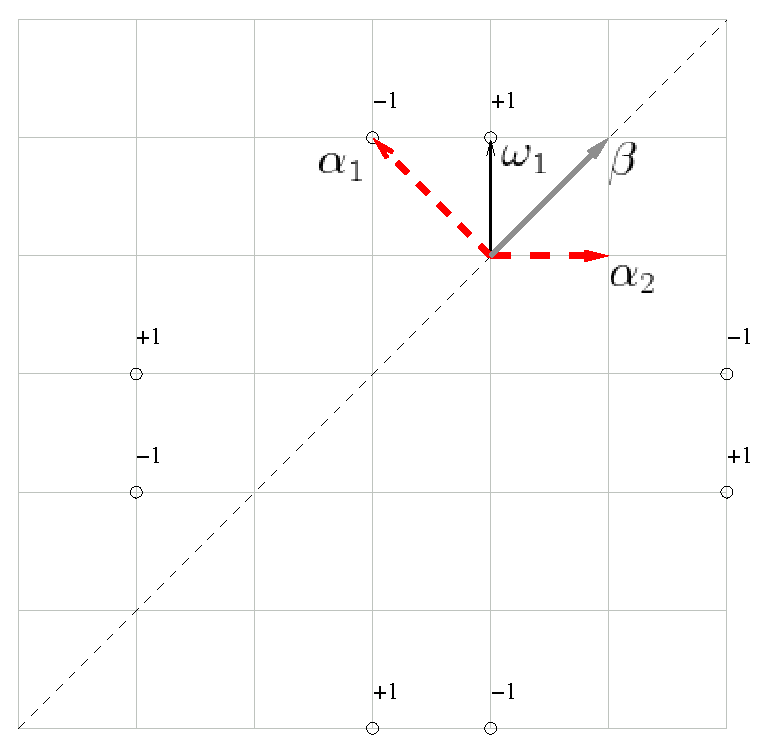
\includegraphics[width=90mm]{B2_A1}
  }
  \caption{Регулярное вложение $A_1$ в $B_2$}
  \label{fig:B2_A1}
\end{figure}
Вот набор аномальных весов $\omega(\mu+\rho)-\rho,\; \omega\in W$ с соответствующими четностями
отражений $\epsilon(\omega)$.
Теперь мы факторизуем группу Вейля $W$ по подгруппе $W_{\bot}=\left\{\omega_1\right\}$. Получаем
следующий набор весов и размерностей представлений  $L^{\pi_{\mathfrak{a}_{\bot}}(\omega(\mu+\rho))-\rho_{\mathfrak{a}_{\bot}}}_{\mathfrak{a}_{\bot}}$:
\begin{figure}[h!tb]
  \noindent\centering{
    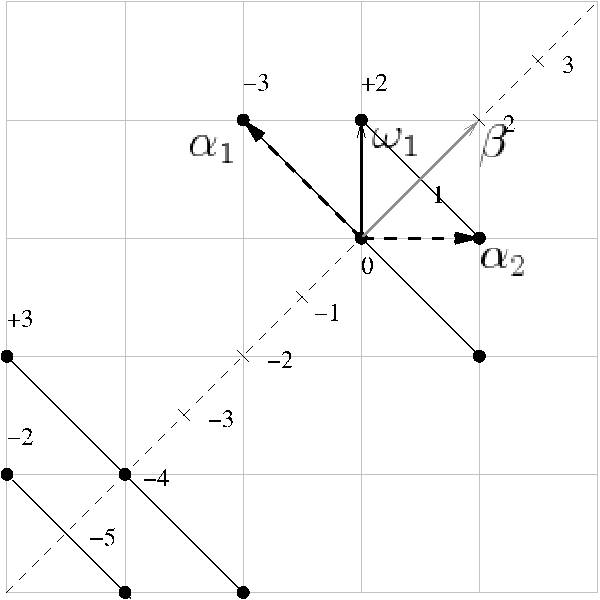
\includegraphics[width=90mm]{B2_A1_2}
  }
  \caption{Аномальные веса и соответствующие $\mathfrak{a}_{\bot}=A_1$-модули}
  \label{fig:B2_A1_2}
\end{figure}

Затем мы проектируем эти веса и размерности на корневое подпространство подалгебры
$\mathfrak{a}=A_1$ и получаем следующие аномальные веса и их кратности:
\begin{equation}
  \label{eq:25}
  (1,2),\; (0,-3),\; (-4,3),\; (-5,-2)
\end{equation}

Аномальный коэффициент ветвления  $k^{(1,0)}_{1}=2$, для коэффициента $k^{(1,0)}_{0}$ из
рекуррентного соотношения получаем
\begin{equation}
  \label{eq:23}
  k^{(1,0)}_{0}=-1\cdot k^{(1,0)}_2 +2\cdot k^{(1,0)}_1 - 3\cdot \delta_{0,0} = 1
\end{equation}

В работе рассмотрено большое число примеров вложений аффинных алгебр Ли. На самом деле мы написали
программу, которая может строить такие примеры автоматически для алгебр Ли не слишком большого
ранга.

Я сейчас покажу результаты применения нашего алгоритма для одного из примеров конформных вложений.

Рассмотрим такое вложение $\mathfrak{a}\subset \mathfrak{g}$, где
$\mathfrak{a}=\hat{A_1}\oplus \hat{A_1}$, а $\mathfrak{g}= \hat{A_3}$. Это
вложение является аффинным расширением специального вложения конечномерных алгебр Ли $A_1\oplus
A_1\subset A3$. ($su(2)\oplus su(2)\subset su(4)$).
\begin{comment}
 Это специальное вложение строится следующим образом: берем четырехмерное
представление $A_1\oplus A_1$ со старшим весом $(1,1)$. Вот веса этого представления
\ref{fig:A_1+A_1_to_A3}, их координаты в базисе фундаментальных весов: $\nu_1=(1,1),\; \nu_2=(-1,1),\; \nu_3=(1,-1),\; \nu_4=(-1,-1)$.

\begin{figure}[h]
  \begin{multicols}{2}
    \hfill
    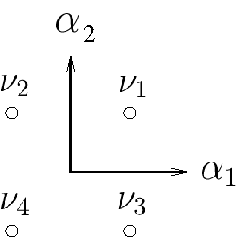
\includegraphics[width=50mm]{A_1+A_1_to_A3}
    \hfill
    \caption{Представление для специального вложения $A_1\oplus A_1\subset A3$}
    \label{fig:A_1+A_1_to_A3}
    \hfill
    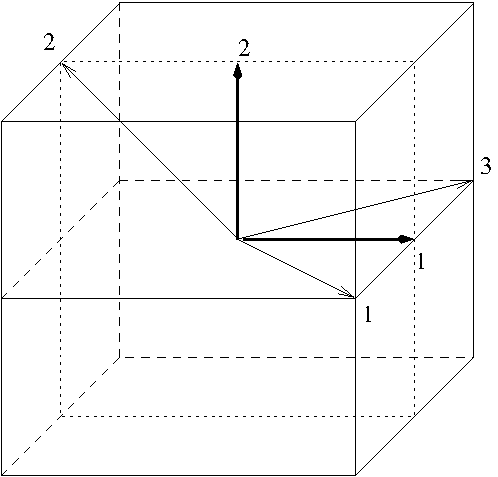
\includegraphics[width=50mm]{A1+A1-A3}
    \hfill
    \caption{Вложенные корни $A_1\oplus A_1\subset A3$}
    \label{fig:A1+A1-A3}
  \end{multicols}
\end{figure}

Тогда матричные элементы представления генераторов подалгебры Картана $b_1,b_2$ в базисе Вейля
даются выражениями
\begin{equation}
  d(b_i)=\mathrm{diag}\left(\frac{2(\nu_1,\alpha_i)}{(\alpha_i,\alpha_i)},\frac{2(\nu_2,\alpha_i)}{(\alpha_i,\alpha_i)},\frac{2(\nu_3,\alpha_i)}{(\alpha_i,\alpha_i)},\frac{2(\nu_4,\alpha_i)}{(\alpha_i,\alpha_i)}\right),
\end{equation}
так что $d(b_1)=\mathrm{diag}(1,-1,1,-1),\;
  d(b_2)=\mathrm{diag}(1,1,-1,-1).$
\end{comment}
Вложенные корни $\alpha_1,\alpha_2$ подалгебры $A_1\oplus A_1$
выражаются через корни $\tilde{\alpha}_i$ алгебры  $A_3$
\begin{equation}
  \label{eq:37}
  \begin{array}{l}
     \alpha_1=\frac{1}{2}(\tilde{\alpha}_1+\tilde{\alpha}_3)\\
     \alpha_2=\frac{1}{2}(\tilde{\alpha}_1+2\tilde{\alpha}_2+\tilde{\alpha}_3)
  \end{array}
\end{equation}
\begin{comment}
Они изображены на рисунке \ref{fig:A1+A1-A3}.
\end{comment}

Вложение имеет индексы  $(2,2)$ и является конформным, так как $c(A_1\oplus A_1)=c(A_1)+c(A_1)=2\frac{x_e \mathrm{dim}(A_1)}{x_e+2}=\frac{\mathrm{dim}A_3}{5}=c(A_3)$.

Для построения модулярно-инвариантной статсуммы нам нужно знать редукцию фундаментальных
представлений $\widehat{su(4)}$. Фундаментальные веса имеют следующие координаты в ортогональном базисе
\begin{equation}
  \begin{array}{lll}
     \omega_0 & = & (0,0,0,0;1;0)\\
     \omega_1 & = & (\frac{3}{4},-\frac{1}{4},-\frac{1}{4},-\frac{1}{4}; 1; 0)\\
     \omega_2 & = & (\frac{1}{2},\frac{1}{2},-\frac{1}{2},-\frac{1}{2}; 1; 0)\\
     \omega_3 & = & (\frac{1}{4},\frac{1}{4},\frac{1}{4},-\frac{3}{4}; 1; 0) \\
  \end{array}
\end{equation}


Множества положительных корней  $\Delta^{+}$ и $\Delta_{\mathfrak{a}}^{+}$:
\begin{equation}
  \label{eq:38}
  \begin{array}{lll}
    \Delta^{+} &=&\left\{\co{\Delta}^{+}=\{\tilde{\alpha}_1, \tilde{\alpha}_2, \tilde{\alpha}_3, \tilde{\alpha}_1+\tilde{\alpha}_2, \tilde{\alpha}_2+\tilde{\alpha}_3, \tilde{\alpha}_1+\tilde{\alpha}_2+\tilde{\alpha}_3\};\right.\\
    &\; & \quad\left.\co{\Delta}+n\delta;\;     +n\delta\;\mbox{с кратностью}\; 3;\; n=1,2,\dots,\right\}\\
    \Delta_{\mathfrak{a}}^{+} &=& \{  \alpha_1,\alpha_2;\;\pm \alpha_1-n\delta,\pm
    \alpha_2-n\delta;\; -n\delta\; \mbox{с кратностью} \; 2;\; n=1,2,\dots\}\\
  \end{array}
\end{equation}

Набор $\Delta^{+}_{\bot}$ пуст.
Веер  $\Gamma _{\frak{a}\subset \frak{g}}$ показан на рисунке \ref{fig:A1+A1-A3_fan}. Конечные координаты
даны в базисе фундаментальных весов $A_1 \oplus A_1$. Элемент $\gamma$ обозначен крестом, если
$s(\gamma)=1$ и кругом, если $s(\gamma)=-1$.
\begin{figure}[h!tb]
  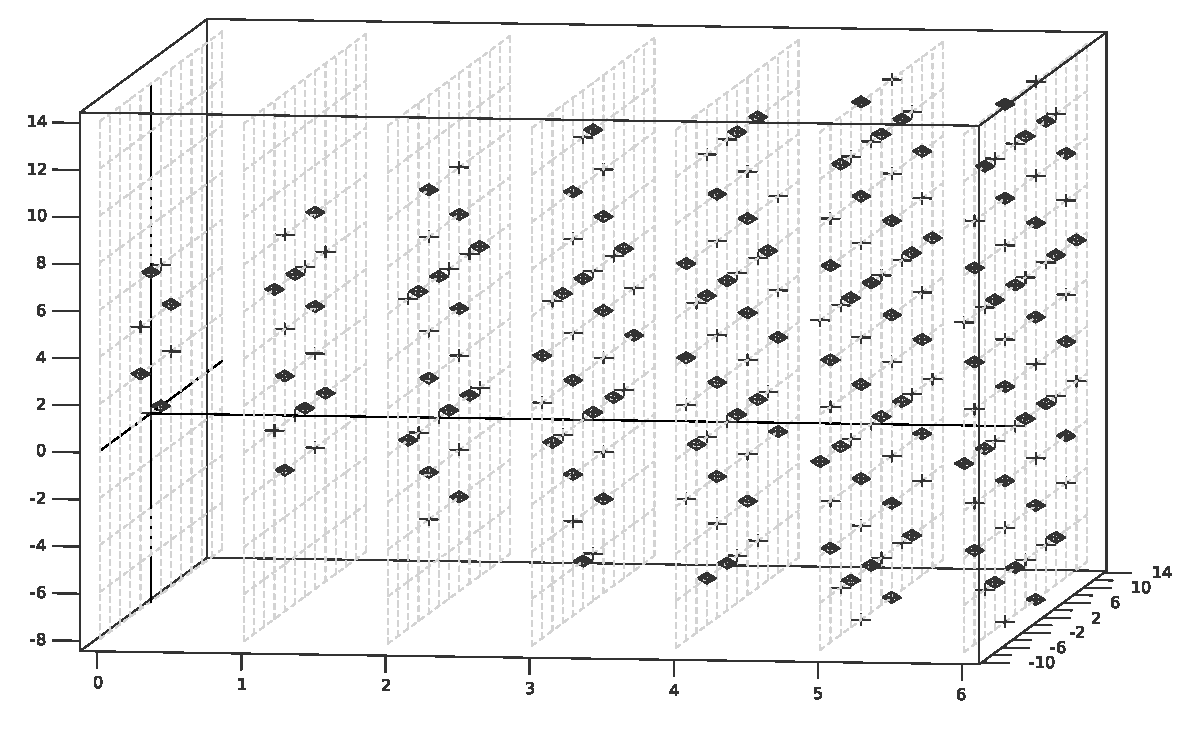
\includegraphics[width=150mm]{A1+A1-A3_fan}
  \caption{Веер для специального вложения $\hat A_1\oplus\hat A_1\subset\hat A_3$}
  \label{fig:A1+A1-A3_fan}
\end{figure}

Мы ограничимся вычислениями до пятого грейда.
\begin{figure}[h!tb]
  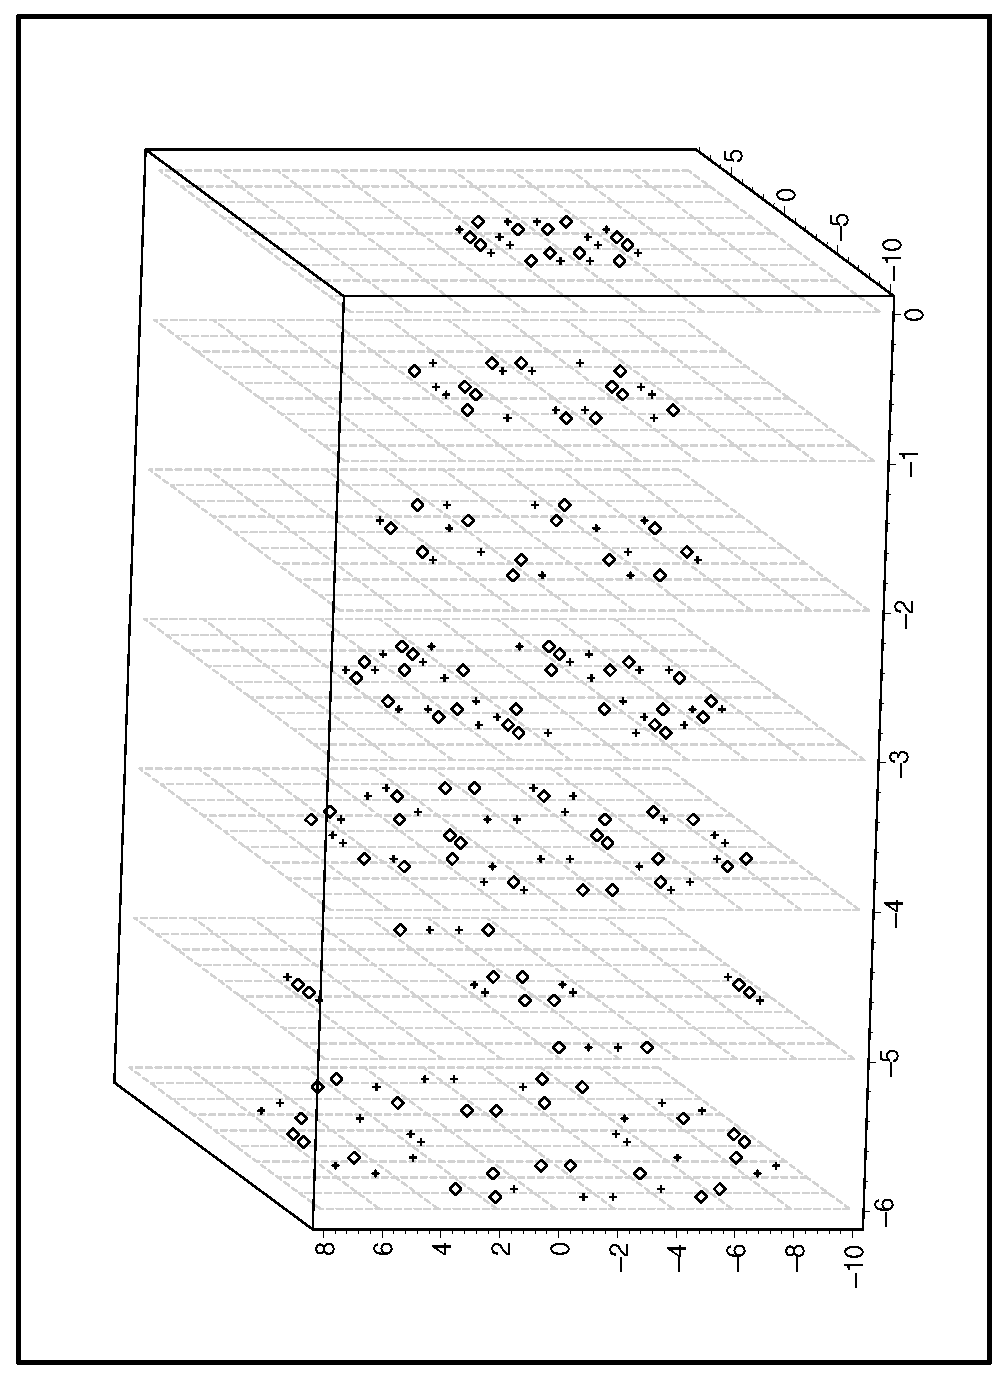
\includegraphics[width=170mm]{A1+A1-A3_anom}
  \caption{Спроектированные аномальные веса $L^{\omega_2}_{A_3}$}
  \label{fig:A1+A1-A3_anom}
\end{figure}

Множество аномальных весов  $\widehat{\Psi^{(\mu)}}=\left\{\omega(\mu+\rho)-\rho;\; \omega\in
  W\right\}$ представления алгебры $\hat{A}_3$ состоит из 192 элементов, их проекции
$\pi_{\mathfrak{a}}\left(\widehat{\Psi^{(\mu)}}\right)$ показаны на рисунке  \ref{fig:A1+A1-A3_anom}
для $\mu=\omega_2=(0,1,0;1;0)$.

Аналогичные картинки для $\omega_0, \omega_1,\omega_3$ я не показываю.

Аномальные коэффициенты ветвления для представления  $L^{(\omega_2)}$ вычислены при помощи
рекуррентных соотношений и показаны на рисунке \ref{fig:A1+A1-A3_branching}. 
\begin{figure}[h!tb]
  \hspace*{-2cm}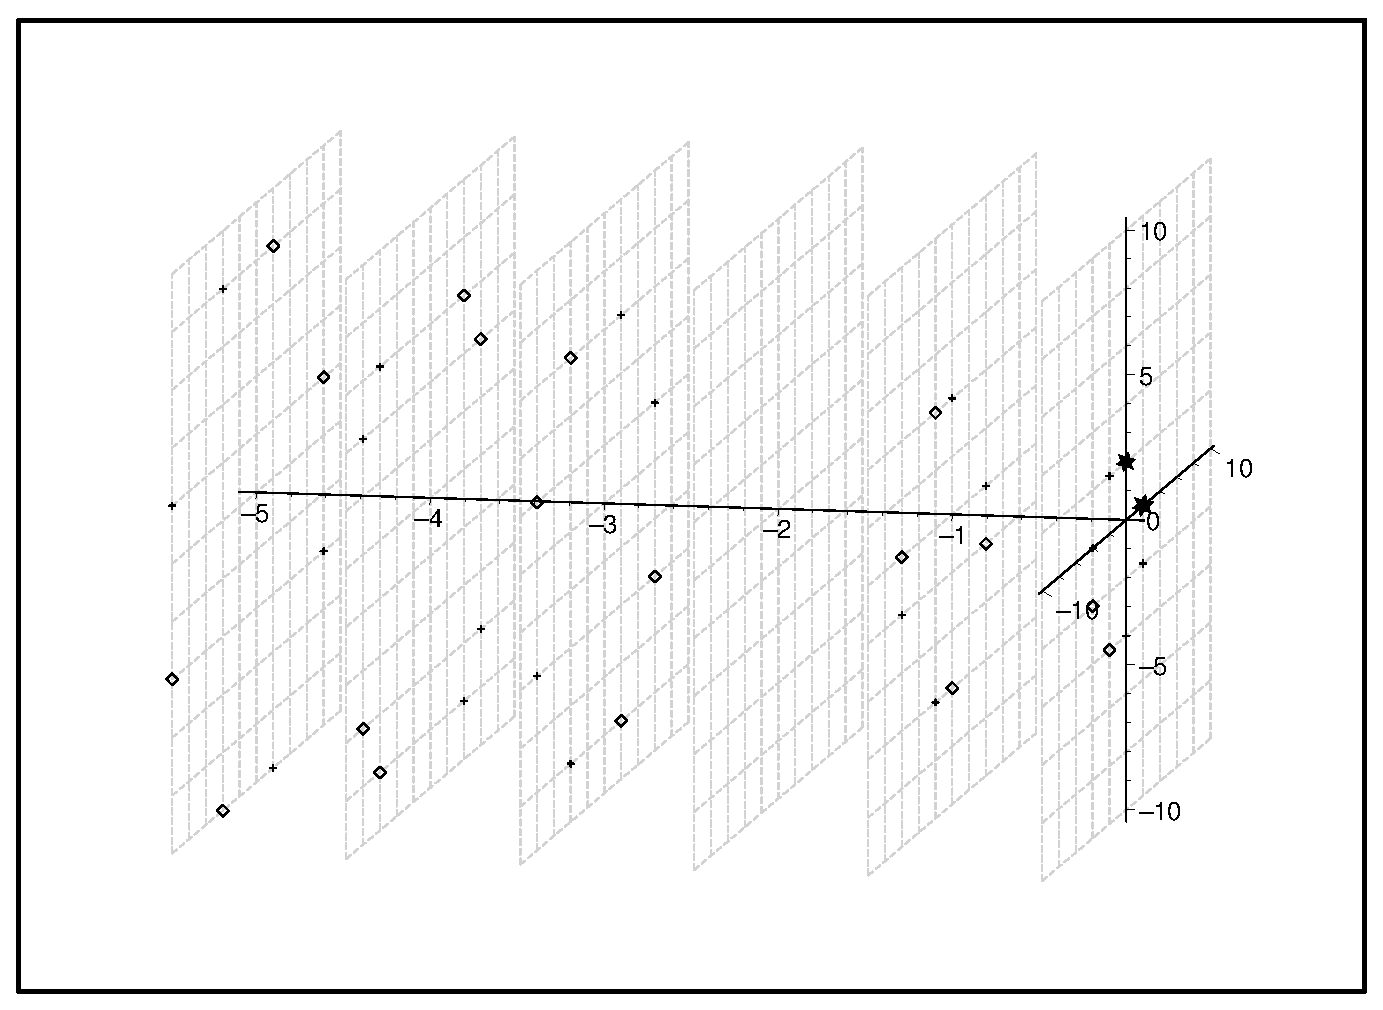
\includegraphics[width=180mm]{A1+A1-A3_branching}
  \caption{Аномальные коэффициенты ветвления для представления $L^{(0,1,0;1;0)}_{A_3}$}
  \label{fig:A1+A1-A3_branching}
\end{figure}

Получаются следующие правила ветвления:
 \begin{equation}
   \label{eq:39}
   \begin{array}{ll}
     L^{(0,0,0;1;0)}_{\hat{A_3}\downarrow \hat{A_1}\oplus \hat{A_1}}= & L_{\hat{A_1}}^{(0;2;0)}\otimes L_{\hat{A_1}}^{(0;2;0)} \\
     L^{(1,0,0;1;0)}_{\hat{A_3}\downarrow \hat{A_1}\oplus \hat{A_1}}= & L_{\hat{A_1}}^{(1;2;0)}\otimes L_{\hat{A_1}}^{(1;2;0)} \\
     L^{(0,1,0;1;0]}_{\hat{A_3}\downarrow \hat{A_1}\oplus \hat{A_1}}= & \left( L_{\hat{A_1}}^{(2;2;0)}\otimes L_{\hat{A_1}}^{(0;2;0)}\right) \oplus \left( L_{\hat{A_1}}^{(0;2;0)}\otimes L_{\hat{A_1}}^{(2;2;0)}\right) \\
     L^{(0,0,1;1;0)}_{\hat{A_3}\downarrow \hat{A_1}\oplus \hat{A_1}}= & L_{\hat{A_1}}^{(1;2;0)}\otimes L_{\hat{A_1}}^{(1;2;0)} \\     
   \end{array}
 \end{equation}

В результате мы получаем модулярно-инвариантную статсумму для WZW-модели с киральной алгеброй $\hat{A}_1\oplus \hat{A}_1$.
\begin{multline}
  \label{eq:40}
  Z=\left|\chi_{(0;2;0)}\chi_{(0;2;0)}\right|^2+2\left|\chi_{(1;2;0)}\chi_{(1;2;0)}\right|^2+ \left|\chi_{(2;2;0)}\chi_{(0;2;0)}+\chi_{(0;2;0)}\chi_{(2;2;0)}\right|^2=\\
  \left|\chi_{(0;2;0)}\right|^4+2\left|\chi_{(1;2;0)}\right|^4+ 4\left|\chi_{(2;2;0)}\chi_{(0;2;0)}\right|^2
\end{multline}

\section{Заключение. Обсуждение перспектив.}
\label{sec:conlusion}

Функции ветвления играют важную роль в coset-моделях. Эти модели строятся путем факторизации
WZW-модели с алгеброй $\mathfrak{g}$ по отношению к модели с подалгеброй $\mathfrak{a}$. Тут функции
ветвления фактически описывают состояния в системе.

Недавно мы заметили, что струнные функции, которые описывают представления, функции ветвления,
описывающие редукцию представлений и функции слияния, которые описывают разложение тензорных
произведений представлений на неприводимые, допускают построение дуальных систем функций. Эти
дуальные функции могут быть построены просто из анализа соответствующих групп и камер Вейля. 
Задача явного построения струнных функций или функций ветвления тогда сведется к обращению матрицы.
Явный вид функций ветвления полезен при изучении coset-моделей. Кроме того, многие
известные результаты могут быть перенесены на дуальные функции, например, результаты Каца о модулярных свойствах
струнных функций и функций ветвления.
В настоящее время мы начали исследовать эти системы дуальных функций. 

Среди других возможных приложений полученных методов можно отметить также приложения в интегрируемых
цепочках, а также в приложения дуальных функций теории модулярных форм. 





\section{Coset-модели}
\label{sec:coset-models}
Ветвления. Функции ветвления и статсуммы. 
Калибровочные WZW-модели. 

\section{SLE}
\label{sec:sle}
SLE на WZW-моделях. Граничные условия. Парафермионы. SLE на coset-моделях.



%%
%% End of file
%%% Local Variables: 
%%% mode: latex
%%% TeX-master: "thesis"
%%% End: 
